
\documentclass[a4paper]{article}

\usepackage[paper=a4paper, left=1.5cm, right=1.5cm, bottom=1.5cm, top=1.5cm]{geometry}
\usepackage[utf8]{inputenc}
\usepackage[spanish]{babel}
\usepackage{ulem}
\usepackage{amssymb, amsmath, amsbsy}
\usepackage{caratula/caratula}
\def\doubleunderline#1{\underline{\underline{#1}}}

\usepackage{tikz}
\usetikzlibrary{bayesnetWLee}

\usepackage{graphicx}
\graphicspath{ {imagenes/} }

\begin{document}

\titulo{Trabajo Práctico \#1 }
\fecha{26 de Mayo de 2016}
\materia{Inferencia Bayesiana}

\integrante{Pedro Rodriguez}{197/12}{pedro3110.jim@gmail.com}
\integrante{Martin Gastón Podavini Rey}{483/12}{marto.rey2006@gmail.com}
% \integrante{Pepe Sánchez}{444/12}{pepe@gmail.com}
% \integrante{Roberto Carlos}{111/10}{roberto@gmail.com}

%Carátula
\maketitle
\newpage

%Indice
\tableofcontents
\newpage

% Demás secciones
%
\section{Introducción}
% \input{introduccion.tex}
En el presente Trabajo Práctico ...


\section{Problema 1 y 3}
Realizamos dos modelos para el problema 1 (caso en el que sabemos que hay una y exactamente una
moneda que esta cargada, con cierta probabilidad), y un modelo para el prolema 3 (cuando cada
moneda esta cargada con probabilidad 0.5). En ambos modelos, la variable determinística $\theta_i$ es un parámetro que dependiendo de si la moneda $i$ esta o no cargada, tiene
cierta distribución, dependiente de las variables $C$ y $NC$ (para cargada y no cargada 
respectivamente). Estas dos variables $C$ y $NC$ son las distribuciones de probabilidad para
una moneda de caer cara cuando esta o no cargada. \\
En el modelo 1a consideramos una variable $p_i$ para 
cada moneda, que define si dicha moneda $i$ esta cargada o no. Esta variable $p_i$ depende de
otra variable, $\alpha$, que tiene distribución uniforme entre cero y la cantidad de monedas. Según el valor entero de esta variable, definimos cuál es la moneda cargada. \\
Por el orto lado, en el modelo 1b, en lugar de hacer uso de un $p_i$ para cada moneda, 
utilizamos un $\alpha_1$ con una distribución categórica, que da a cada moneda una misma
probabilidad de estar cargada. \\
Las variables $\alpha$ respresentan nuestro prior sobre la probabilidad de que cada moneda $i$
este o no cargada. \\
Finalmente, en el modelo 2 (para el problema 3), el $alpha_{2_i}$ tiene distribución 
Bernoulli(0.5), para modelar que cada moneda esta cargada con probabilidad 0.5. En este caso, modificamos levemente el modelo respecto al anterior. \\


\subsection{Modelo 1a}
\tikz{ %
		\node[obsDisc] (m) {$m_i$} ; %
        \node[detCont, right=of m] (theta) {$\theta_i$} ; %
        \node[detCont, right=of theta] (p) {$p_i$} ; %

		\node[latentCont, above left=of theta] (C) {$C$} ;
		\node[latentCont, above right=of theta] (NC) {$NC$} ;
		\node[latentCont, right=of p] (alpha) {$\alpha$} ;

     	\edge[] {theta} {m} ; 
     	\edge[] {p} {theta} ;
     	\edge[] {C} {theta} ;
     	\edge[] {NC} {theta} ;
     	\edge[] {alpha} {p} ;
        \plate {} { (m) (theta) (p) } {$i=1 \dots cantMonedas$}; %
}
\newline
Likelihood y priors: \\
\begin{itemize}
	\item $ m_i \sim Binomial(\theta_i, cantLanzamientos) $
	\item $ C \sim Beta(k_1, k_1) $, con $k_1$ una constante grande ( $\geq 100 $ )
	\item $ NC \sim Beta(k_2, k_2) $, con $k_2$ una con constante entre 0 y 1 
	\item $ \alpha \sim Uniforme(0,cantMonedas) $
	\item $ \theta_i = p_i * C + (1 - p_i) * NC $
	\item $ p_i = (\alpha < i \leq \alpha + 1) $
\end{itemize}



\subsection{Modelo 1b}
\tikz{ %
		\node[obsDisc] (m) {$m_i$} ; %
        \node[detCont, right=of m] (theta) {$\theta_i$} ; %

		\node[latentCont, above left=of theta] (C) {$C$} ;
		\node[latentCont, above right=of theta] (NC) {$NC$} ;
		\node[latentCont, right=of theta] (alpha) {$\alpha_1$} ;

     	\edge[] {theta} {m} ;
     	\edge[] {C} {theta} ;
     	\edge[] {NC} {theta} ;
     	\edge[] {alpha} {theta} ;
        \plate {} { (m) (theta) } {$i=1 \dots cantMonedas$}; %
}
\newline
Likelihood y priors: \\
\begin{itemize}
	\item $ m_i \sim Binomial(\theta_i, cantLanzamientos) $
	\item $ C \sim Beta(k_1, k_1) $, con $k_1$ una constante grande ( $\geq 100 $ )
	\item $ NC \sim Beta(k_2, k_2) $, con $k_2$ una con constante entre $0$ y $1$
	\item $ \alpha_1 \sim Categorica(\dfrac{1}{cantMonedas}, \dots , \dfrac{1}{cantMonedas}) $
	\item $ \theta_i = (i = \alpha_1) $
\end{itemize}

\subsection{Modelo 2a}
\tikz{ %
		\node[obsDisc] (m) {$m_i$} ; %
        \node[detCont, right=of m] (theta) {$\theta_i$} ; %

		\node[latentCont, above left=of theta] (C) {$C$} ;
		\node[latentCont, above right=of theta] (NC) {$NC$} ;
		\node[latentCont, right=of theta] (alpha) {$\alpha_{2_i}$} ;

     	\edge[] {theta} {m} ;
     	\edge[] {C} {theta} ;
     	\edge[] {NC} {theta} ;
     	\edge[] {alpha} {theta} ;
        \plate {} { (m) (theta) (alpha)} {$i=1 \dots cantMonedas$}; %
}
\newline
Likelihood y priors: en este caso, el likelihood y los priors son los mismos que en el modelo 1a,
cambiando $\alpha_1$ 
por $\alpha_2$:
\begin{itemize}
	\item $ \alpha_{2_i} \sim Bernoulli(0.5) $
\end{itemize}

\section {Problema 2}
En esta sección, mostramos la inferencia y muestras a posteriori hechas sobre los 
parámetros que son interesantes de
observar en cada uno de los modelos, como $theta_i$ (para cada moneda) y $alpha$
(la probabilidad de cada moneda de estar cargada). \\
Para entender los gráficos: cuando decimos que priorcargada $= x$ o que 
priornocargada $= y$, nos referimos que que $C \sim Beta(x,x)$ y a que 
$NC \sim Beta(y,y)$ respectivamente. \\

A continuación, exponemos para el Modelo 1, y para los datos del enunciado,
las probabilidades posteriores de cada moneda de estar cargadas. Tomamos 
$priorcargada = 0.4$, para modelar que cuando una moneda esta cargada, nos 
referimos a que lo más probable es que esta cargada con desvío hacia alguno
de los dos lados (cara o ceca), y elegimos $priornocargada = 100$, para 
modelar cuán fuerte es nuestra creencia a priori de que una moneda no está cargada si
decimos que no lo está. \\

Se puede ver que según el Modelo 1a y 1b, lo más probable es por mucho que la moneda número
3 (la que salió todas las veces cara), sea la que está cargada. 

\subsection{ }

\begin{figure}[h!]
\centering
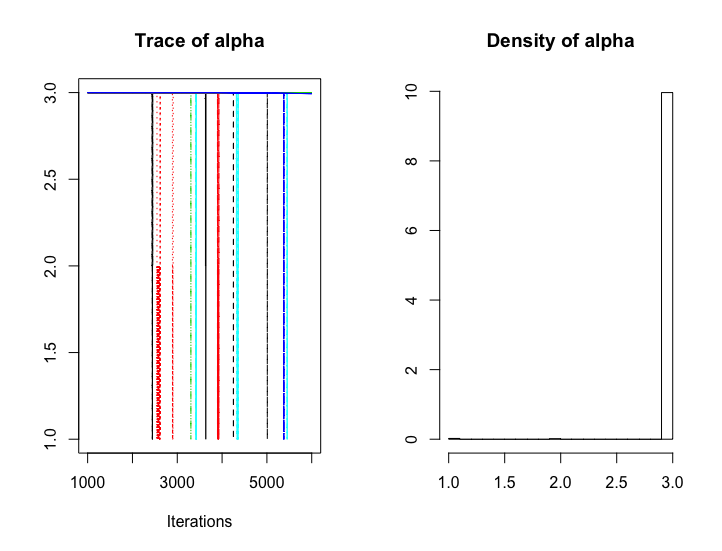
\includegraphics[scale=0.5] {img5.png}
\caption{ Histograma para probabilidades posteriores de cada moneda en el Modelo 1,
			los datos del enunciado }
\end{figure}

En los próximos gráficos se puede observar que al utilizar el modelo 1 (según el cuál
sólo una de las monedas está cargada), si cambiamos los resutlados obtenidos (3, 4 y 10 caras vs.
4, 9 y 10 caras), hay sólo una de las monedas que en la posteriori muestra altas probabilidades de estar cargada. En el caso segundo caso (cuando la segunda y tercer moneda caen 9 y 10 veces cara cada una), se observa que la segunda moneda (la que cayó menos veces cara de las dos) y no la tercera, presenta una cola más larga, mostrando así que su probabilidad de estar cargada es levemente más alta que si los resultados obtenidos hubieran sido los otros. \\

En la siguiente figura, la media reportada para cada uno de los $theta_i$ de cada moneda son:
$0.4860157$ , $0.486702$ y $0.958525$ , mientras que los desvíos estándar de cada una son
$0.03661387$ , $0.03459539$ y $0.06977161$.

\begin{figure}[h!]
\centering
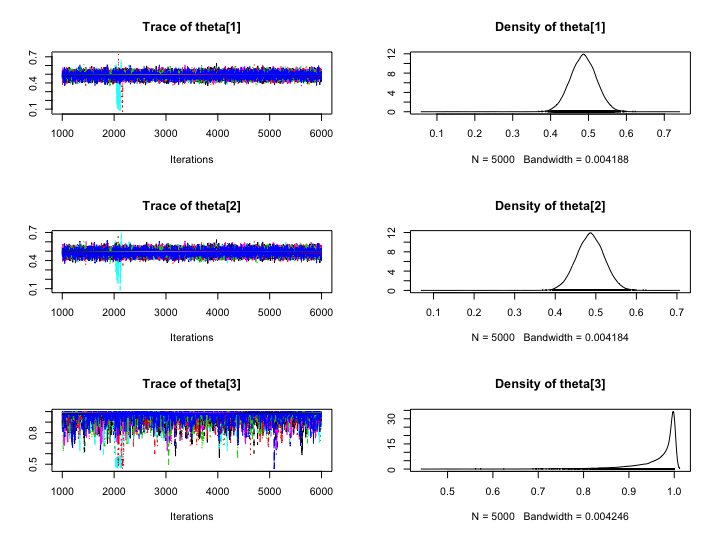
\includegraphics[scale=0.5] {img1.png}
\caption{Modelo 1a y 1b : resultados = (3,4,10), priorcargada=.4, priornocargada=100 }
\end{figure}

En la siguiente figura, la media reportada para cada uno de los $theta_i$ de cada moneda son:
$0.5136371$ , $0.5290319$ y $0.9422637$ , mientras que los desvíos estándar de cada una son
$0.03440065$ , $0.08164135$ y $0.1079074$. Se puede ver que, como nuestro modelo restringe que
sólo puede haber una de las monedas cargada, se toma la moneda que más probabilidades tiene de
ser la cargada según los datos y esa es la única que presenta una densidad de probabilidad 
sesgada respecto de las densidades de probabilidad a posteriori del resto de las monedas.

\begin{figure}[h!]
\centering
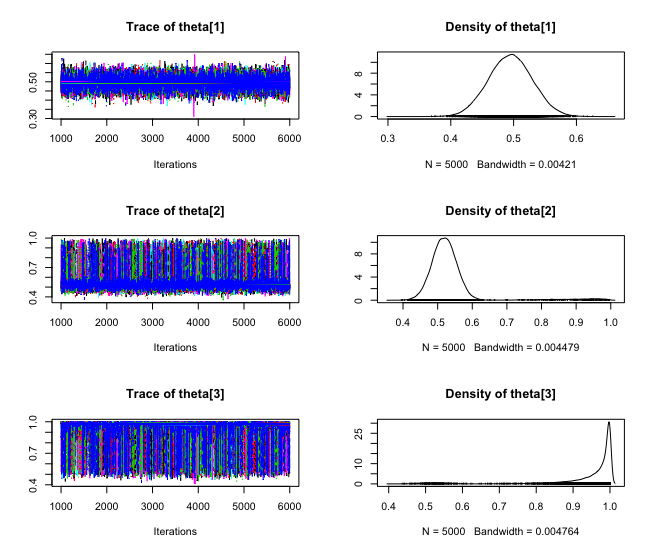
\includegraphics[scale=0.5] {img2.png}
\caption{Modelo 1a y 1b : resultados = (4,9,10), priorcargada=.4, priornocargada=100 }
\end{figure}


\subsection{ }
A continuación, probamos variar las priors sobre $C$ y $NC$, para ver como influyen
en la posteriori de $\alpha$. La media reportada para cada una de las monedas $m_i$ son:
$0.4992888$ , $0.5000426$ y $0.50325$ , mientras que los desvíos estándar de cada una son
$0.0145012$ , $0.014499$ y $0.014323$. Se puede ver que al cambiar los priors, para los 
mismos datos que en la Figura 1, obtenemos resultados muy diferentes.

\begin{figure}[h!]
\centering
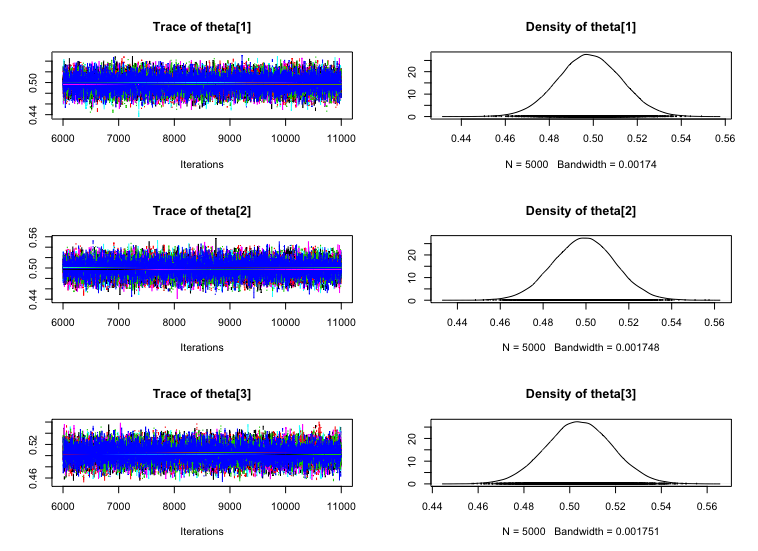
\includegraphics[scale=0.5] {img4.png}
\caption{ Modelo 1b : resultados = (3,4,10), priorcargada=600, priornocargada=600 }
\end{figure}

\begin{figure}[h!]
\centering
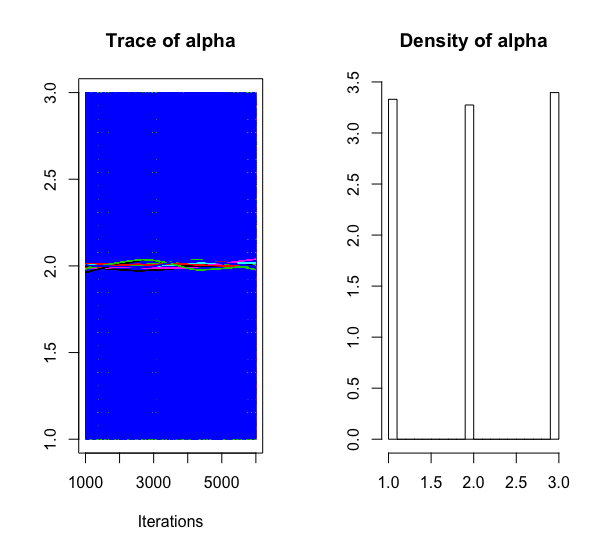
\includegraphics[scale=0.5] {img3.png}
\caption{ Histograma : resultados = (3,4,10), priorcargada=600, priornocargada=600 }
\end{figure}

\subsection{ }
Finalmente, veamos qué sucede cuando en el modelo permitimos que cada moneda esté cargada, con
probabilidad $0.5$ para los datos (3,4,10) y (4,9,10).

La media reportada para cada uno de los $theta_i$ de cada moneda para los datos (3,4,10) son:
$0.4352866$ , $0.4777972$ y $0.960523$ , mientras que los desvíos estándar de cada una son
$0.1152681$ , $08022269$ y $0.06531687$. También puede apreciarse que la primera moneda, que
en los datos presento 3 caras vs. 4 caras para la segunda moneda, tiene mayores probabilidades
de ser la que está cargada hacia la izquierda que la segunda moneda.

\begin{figure}[h!]
\centering
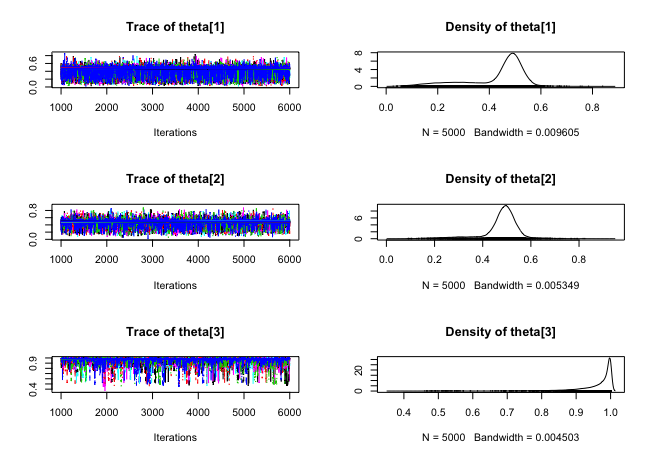
\includegraphics[scale=0.5] {img7.png}
\caption{ Modelo 2 : resultados = (3,4,10), priorcargada=0.4, priornocargada=100 }
\end{figure}

La media reportada para cada uno de los $theta_i$ de cada moneda para los datos (4,9,10) son:
$0.4770534$ , $0.830595$ y $0.9609804$ , mientras que los desvíos estándar de cada una son
$0.08123214$ , $0.1453149$ y $0.06049837$.

\begin{figure}[h!]
\centering
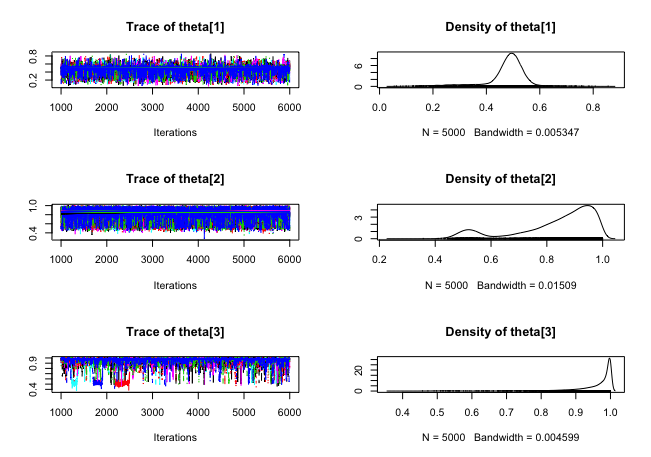
\includegraphics[scale=0.5] {img6.png}
\caption{ Modelo 2 : resultados = (4,9,10), priorcargada=0.4, priornocargada=100 }
\end{figure}

En los gráficos precedentes, se puede apreciar claramente la diferencia de las probabilidades
a posteriori inferidas por los diferentes modelos, si se los compara con los 
gráficos que presentamos en las figuras anteriores para los mismos datos pero con el 
primer modelo.

\newpage
\section {Problema 4}
Llamamos $ y = ( y_1 \dots y_n ) $. \\

Aquí, $ p(\theta | y) $ es la posterior predictive que obtenemos tras las primeras
$ y_1 \dots y_n $ observaciones para cada moneda. \\

$ 
p(y_{n+1} | y) =  \int p(y_{n+1}, \theta | y) d\theta 
			   =  \int p(y_{n+1} | y, \theta) p(\theta | y) d \theta
			   =  \int p(y_{n+1} | \theta) p(\theta | y) d \theta
			   =  \int \theta^{y_{n+1}} (1 - \theta)^{1 - y_{n+1}} p(\theta | y) d \theta
$

%
%
% \section{Conclusiones}
% \input{conclusiones.tex}
%

\end{document}

